%--------------------------------------------------
%   D O C U M E N T   C O N F I G U R A T I O N
%--------------------------------------------------

\newcolumntype{C}[1]{>{\centering\arraybackslash}p{#1}}

%--------------------------------------------------
%         D O C U M E N T   C O N T E N T
%--------------------------------------------------

\section{Graphical User Interface}
\noindent The Graphical User Interface is fully designed and implemented in Unity game engine version 5.4.1f1 Personal. Only standard unity assets are used, no additional elements are required. All of the implementation is written in C\# programming language.

\subsection{EPIC 1 Specific Information}\label{gui-epic1-info}
\noindent In EPIC 1 all of the users are gathered on the same device and all of the user actions are performed with this device's mouse and keyboard. The Graphical User Interface of this version looks as follows:

\begin{figure}[h]\label{gui-epic1}\centering
	\includegraphics[scale=1, frame]{gui-imgs/GUI-epic1}
	\caption{EPIC 1 Graphical User Interface}
\end{figure}

\subsection{Palette of colors}
\noindent The full spectrum of colors that are used in the project is presented below.

\vspace*{-0.125cm}
\begin{figure}[!h]\label{gui-colors}\centering
	\captionsetup{justification=centering}
	\begin{subfigure}{0.105\textwidth}\centering
		\includegraphics[scale=1, frame]{gui-imgs/R46G49B56A255}
		\vspace*{-20px}\caption*{\hspace*{-0.25px}\tiny R46 G49 B56 \\ \tiny A255}
	\end{subfigure}
	\begin{subfigure}{0.105\textwidth}\centering
		\includegraphics[scale=1, frame]{gui-imgs/R69G73B84A64}
		\vspace*{-20px}\caption*{\hspace*{-0.25px}\tiny R69 G73 B84 \\ \tiny A64}
	\end{subfigure}
	\begin{subfigure}{0.105\textwidth}\centering
		\includegraphics[scale=1, frame]{gui-imgs/R69G73B84A255}
		\vspace*{-20px}\caption*{\hspace*{-0.25px}\tiny R69 G73 B84 \\ \tiny A255}
	\end{subfigure}
 	\begin{subfigure}{0.105\textwidth}\centering
		\includegraphics[scale=1, frame]{gui-imgs/R51G153B255A64}
		\vspace*{-20px} \caption*{\hspace*{-0.25px}\tiny R153 G0 B255 \\ \tiny A264}
	\end{subfigure}
	\begin{subfigure}{0.105\textwidth}\centering
		\includegraphics[scale=1, frame]{gui-imgs/R255G153B102A64}
		\vspace*{-20px} \caption*{\hspace*{-0.25px}\tiny R51 G153 B255 \\ \tiny A64}
	\end{subfigure}
	\begin{subfigure}{0.105\textwidth}\centering
		\includegraphics[scale=1, frame]{gui-imgs/R255G153B102A255}
		\vspace*{-20px} \caption*{\hspace*{-0.25px}\tiny R255 G153 B102 \\ \tiny A255}
	\end{subfigure}
 	\begin{subfigure}{0.105\textwidth}\centering
		\includegraphics[scale=1, frame]{gui-imgs/R51G153B255A255}
		\vspace*{-20px} \caption*{\hspace*{-0.25px}\tiny R51 G153 B255 \\ \tiny A255}
	\end{subfigure}
	\begin{subfigure}{0.105\textwidth}\centering
		\includegraphics[scale=1, frame]{gui-imgs/R153G0B255A255}
		\vspace*{-20px} \caption*{\hspace*{-0.25px}\tiny R153 G0 B255 \\ \tiny A255}
	\end{subfigure}
	\begin{subfigure}{0.105\textwidth}\centering
		\includegraphics[scale=1, frame]{gui-imgs/R153G0B255A64}
		\vspace*{-20px} \caption*{\hspace*{-0.25px}\tiny R153 G0 B255 \\ \tiny A64}
	\end{subfigure} \\
	\begin{subfigure}{0.105\textwidth}\centering
		\includegraphics[scale=1, frame]{gui-imgs/R214G0B147A64}
		\vspace*{-20px}\caption*{\hspace*{-0.25px}\tiny R214 G0 B147 \\ \tiny A64}
	\end{subfigure}
	\begin{subfigure}{0.105\textwidth}\centering
		\includegraphics[scale=1, frame]{gui-imgs/R214G0B147A255}
		\vspace*{-20px} \caption*{\hspace*{-0.25px}\tiny R214 G0 B147 \\ \tiny A255}
	\end{subfigure}
	\begin{subfigure}{0.105\textwidth}\centering
		\includegraphics[scale=1, frame]{gui-imgs/R0G204B153A64}
		\vspace*{-20px} \caption*{\hspace*{-0.25px}\tiny R0 G204 B153 \\ \tiny A64}
	\end{subfigure}
	\begin{subfigure}{0.105\textwidth}\centering
		\includegraphics[scale=1, frame]{gui-imgs/R0G204B153A255}
		\vspace*{-20px} \caption*{\hspace*{-0.25px}\tiny R0 G204 B153 \\ \tiny A255}
	\end{subfigure}
	\begin{subfigure}{0.105\textwidth}\centering
		\includegraphics[scale=1, frame]{gui-imgs/R102G255B102A255}
		\vspace*{-20px} \caption*{\hspace*{-0.25px}\tiny R102 G255 B102 \\ \tiny A255}
	\end{subfigure}
	\begin{subfigure}{0.105\textwidth}\centering
		\includegraphics[scale=1, frame]{gui-imgs/R102G255B102A64}
		\vspace*{-20px} \caption*{\hspace*{-0.25px}\tiny R102 G255 B102 \\ \tiny A64}
	\end{subfigure}
	\begin{subfigure}{0.105\textwidth}\centering
		\includegraphics[scale=1, frame]{gui-imgs/R0G204B153A64}
		\vspace*{-20px} \caption*{\hspace*{-0.25px}\tiny R255 G153 B102 \\ \tiny A64}
	\end{subfigure}
	\begin{subfigure}{0.105\textwidth}\centering
		\includegraphics[scale=1, frame]{gui-imgs/R255G255B255A255}
		\vspace*{-20px}\caption*{\hspace*{-0.25px}\tiny R255 G255 B255 \\ \tiny A255}
	\end{subfigure}
	\begin{subfigure}{0.105\textwidth}\centering
		\includegraphics[scale=1]{gui-imgs/R255G255B255A255}
	\end{subfigure}
	\caption{Pallete of colors}
\end{figure}

\subsection{Components}\label{gui-components}
\noindent The Graphical User Interface is build with standard unity UI objects. These objects are built into components that make up the user interface.\\

\dirtree{%
.1 \hyperref[gui-playersettingspanel]{PlayerSettingsPanel} [Canvas].
.2 \hyperref[gui-playerdisabledpanel]{PlayerDisabledPanel} [Button].
.3 PlayerNicknameInputField [InputField].
.2 \hyperref[gui-playerenabledpanel]{PlayerEnabledPanel} [Panel].
.3 PlayerNicknameInputField [InputField].
.3 PlayerDisableButton [Button].
.3 PlayerKeyLeftButton [Button].
.3 PlayerKeyRightButton [Button].
.2 \hyperref[gui-arenasizepanel]{ArenaSizePanel} [Panel].
.3 ArenaSizeTextPanel [Panel].
.4 ArenaSizeText [Text].
.3 ArenaSizeSlider [Slider].
.2 \hyperref[gui-initialspeedpanel]{InitialSpeedPanel} [Panel].
.3 InitialSpeedTextPanel [Panel].
.4 InitialSpeedText [Text].
.3 InitialSpeedSlider [Slider].
.2 \hyperref[gui-initialsizepanel]{InitialSizePanel} [Panel].
.3 InitialSizeTextPanel [Panel].
.4 InitialSizeText [Text].
.3 InitialSizeSlider [Slider].
.2 \hyperref[gui-startbutton]{StartButton} [Button].
}

\subsubsection{PlayerSettingsPanel}\label{gui-playersettingspanel}
\noindent The main GUI canvas object. It is the user interface background on which all other components are placed. The \cprotect{\hyperref[gui-colors]}{\verb|R46 G49 B56 A255|} value is used as its color. The panel size is \verb|650x457| pixels.

\begin{table}[h!]\centering
	\caption{PlayerSettingsPanel details}
	\begin{tabular}{|C{4cm}|C{4cm}|C{4cm}|C{4cm}|}
		\hline
		\textbf{Name} & \textbf{UI object} & \textbf{Size} & \textbf{Color (RGBA)} \\\hline
		PlayerSettingsPanel & Canvas & 650x475px & \hyperref[gui-colors]{46,49,56,255} \\\hline
	\end{tabular}
\end{table}

\subsubsection{PlayerDisabledPanel}\label{gui-playerdisabledpanel}
\noindent Unity \verb|Button| object which is used to add a player to the game. Its text font is Arial of size 55 and color \cprotect{\hyperref[gui-colors]}{\verb|R255 G255 B255 A255|}. The button consist of \verb|PlayerNicknameInputField| subcomponent.

\vspace*{-.25cm}
\begin{figure}[h!]\centering
	\hspace*{.75cm}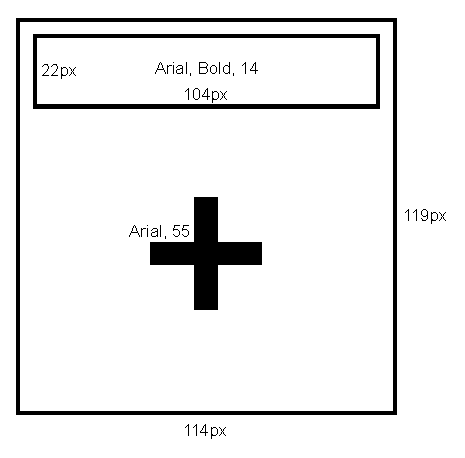
\includegraphics[scale=1]{gui-imgs/playerdisabledpanel-size}
	\caption{PlayerDisabledPanel size}
\end{figure}

\begin{table}[h!]\centering
	\caption{PlayerDisabledPanel details}
	\begin{tabular}{|C{4cm}|C{4cm}|C{4cm}|C{4cm}|}
		\hline
		\textbf{Name} & \textbf{UI object} & \textbf{Size} & \textbf{Color (RGBA)} \\\hline
		PlayerDisabledPanel & Button & 114x119px & \hyperref[gui-colors]{69,73,84,64} \\\hline
		PlayerNicknameInputField & InputField & 104x22px & \hyperref[gui-colors]{214,0,147,64} \\
		& & & \hyperref[gui-colors]{153,0,255,64} \\
		& & & \hyperref[gui-colors]{51,153,255,64} \\
		& & & \hyperref[gui-colors]{255,153,102,64} \\
		& & & \hyperref[gui-colors]{0,204,153,64} \\
		& & & \hyperref[gui-colors]{102,255,102,64} \\\hline
	\end{tabular}
\end{table}

\noindent The ingame pictures of all possible PlayerDisabledPanels look as follows:

\begin{figure}[h!] 
	\centering
	\begin{subfigure}{0.185\textwidth}
		\centering
		\includegraphics[scale=1, frame]{gui-imgs/player1disabledpanel}
	\end{subfigure}
	\begin{subfigure}{0.185\textwidth}
		\centering
		\includegraphics[scale=1, frame]{gui-imgs/player2disabledpanel}
	\end{subfigure}
	\begin{subfigure}{0.185\textwidth}
		\centering
		\includegraphics[scale=1, frame]{gui-imgs/player3disabledpanel}
	\end{subfigure} \\
	\begin{subfigure}{0.185\textwidth}
		\centering
		\includegraphics[scale=1, frame]{gui-imgs/player4disabledpanel}
	\end{subfigure}
	\begin{subfigure}{0.185\textwidth}
		\centering
		\includegraphics[scale=1, frame]{gui-imgs/player5disabledpanel}
	\end{subfigure}
	\begin{subfigure}{0.185\textwidth}
		\centering
		\includegraphics[scale=1, frame]{gui-imgs/player6disabledpanel}
	\end{subfigure}
	\caption{PlayerDisabledPanels ingame}
\end{figure}

\noindent The component functionality is explained in the \hyperref[gui-implementation]{implementation} section.

\subsubsection{PlayerEnabledPanel}\label{gui-playerenabledpanel}
\noindent Activated version of the \cprotect{\hyperref[gui-playerdisabledpanel]}{\verb|PlayerDisabledPanel|}. Consists of four subcomponents: \verb|PlayerNicknameInputField|, \verb|PlayerDisableButton|, \verb|PlayerKeyLeftButton|, \verb|PlayerRightLeftButton|.

\begin{figure}[h!]\centering
	\hspace*{.75cm}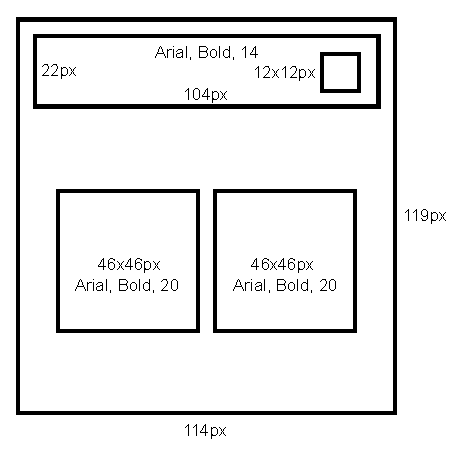
\includegraphics[scale=1]{gui-imgs/playerenabledpanel-size}
	\caption{PlayerEnabledPanel size}
\end{figure}

\newpage
\begin{table}[h!]\centering
	\caption{PlayerEnabledPanel details}
	\begin{tabular}{|C{4cm}|C{4cm}|C{4cm}|C{4cm}|}
		\hline
		\textbf{Name} & \textbf{UI object} & \textbf{Size} & \textbf{Color (RGBA)} \\\hline
		PlayerEnabledPanel & Button & 114x119px & \hyperref[gui-colors]{69,73,84,255} \\\hline
		PlayerNicknameInputField & InputField & 104x22px & \hyperref[gui-colors]{214,0,147,255} \\
		& & & \hyperref[gui-colors]{153,0,255,255} \\
		& & & \hyperref[gui-colors]{51,153,255,255} \\
		& & & \hyperref[gui-colors]{255,153,102,255} \\
		& & & \hyperref[gui-colors]{0,204,153,255} \\
		& & & \hyperref[gui-colors]{102,255,102,255} \\\hline
		PlayerDisableButton & Button & 12x12px & \hyperref[gui-colors]{255,255,255,255} \\\hline
		PlayerKeyLeftButton & Button & 46x46px & \hyperref[gui-colors]{46,49,56,255} \\\hline
		PlayerRightLeftButton & Button & 46x46px & \hyperref[gui-colors]{46,49,56,255} \\\hline
	\end{tabular}
\end{table}

\noindent The ingame pictures of all possible PlayerEnabledPanels look as follows:

\begin{figure}[h!] 
	\centering
	\begin{subfigure}{0.195\textwidth}
		\centering
		\includegraphics[scale=1, frame]{gui-imgs/player1enabledpanel}
	\end{subfigure}
	\begin{subfigure}{0.195\textwidth}
		\centering
		\includegraphics[scale=1, frame]{gui-imgs/player2enabledpanel}
	\end{subfigure}
	\begin{subfigure}{0.195\textwidth}
		\centering
		\includegraphics[scale=1, frame]{gui-imgs/player3enabledpanel}
	\end{subfigure} \\
	\begin{subfigure}{0.195\textwidth}
		\centering
		\includegraphics[scale=1, frame]{gui-imgs/player4enabledpanel}
	\end{subfigure}
	\begin{subfigure}{0.195\textwidth}
		\centering
		\includegraphics[scale=1, frame]{gui-imgs/player5enabledpanel}
	\end{subfigure}
	\begin{subfigure}{0.195\textwidth}
		\centering
		\includegraphics[scale=1, frame]{gui-imgs/player6enabledpanel}
	\end{subfigure}
	\caption{PlayerEnabledPanels ingame}
\end{figure}

\noindent All of the componetns has its default values hardcoded. All of them along with functionalities are explained in the \hyperref[gui-implementation]{implementation} section.

\subsubsection{ArenaSizePanel}\label{gui-arenasizepanel}
\noindent Consists of two subcomponents: \verb|ArenaSizeTextPanel| with the "ARENA SIZE" \verb|ArenaSizeText| written in capitals letters only and \verb|ArenaSizeSlider| with three possible values.

\begin{figure}[h!]\centering
	\hspace*{.75cm}\includegraphics[scale=1]{gui-imgs/arenasizepanel-size}
	\caption{ArenaSizePanel size}
\end{figure}

\newpage
\begin{table}[h!]\centering
	\caption{ArenaSizePanel details}
	\begin{tabular}{|C{4cm}|C{4cm}|C{4cm}|C{4cm}|}
		\hline
		\textbf{Name} & \textbf{UI object} & \textbf{Size} & \textbf{Color (RGBA)} \\\hline
		ArenaSizePanel & Panel & 155x58px & \hyperref[gui-colors]{69,73,84,255} \\\hline
		ArenaSizeTextPanel & Panel & 164x22px & \hyperref[gui-colors]{46,49,56,255} \\\hline
		ArenaSizeText & Text & Arial, 14 & \hyperref[gui-colors]{255,255,255,255} \\\hline
		ArenaSizeSlider & Slider & 115x6px & \hyperref[gui-colors]{255,255,255,255} \\
		& & & \hyperref[gui-colors]{0,255,153,255} \\\hline
	\end{tabular}
\end{table}

\noindent The ingame pictures of the component looks as follows:

\begin{figure}[h] 
	\centering
	\begin{subfigure}{0.2\textwidth}\centering
		\includegraphics[scale=1, frame]{gui-imgs/slider0}
	\end{subfigure}
	\begin{subfigure}{0.2\textwidth}\centering
		\includegraphics[scale=1, frame]{gui-imgs/slider1}
	\end{subfigure}
	\caption{InGame ArenaSizePanel Slider}
\end{figure}

\begin{figure}[h!] 
	\centering
	\includegraphics[scale=1, frame]{gui-imgs/arenasizepanel}
	\caption{ArenaSizePanel ingame}
\end{figure}

\noindent The functionality and implemetation of \verb|ArenaSizePanel| is described in the \hyperref[gui-implementation]{implementation} section.

\subsubsection{InitialSpeedPanel}\label{gui-initialspeedpanel}
\noindent Simiar to \cprotect{\hyperref[gui-arenasizepanel]}{\verb|ArenaSizePanel|}. The only differece is \verb|InitialSpeedText| which now is "PLAYERS SPEED".

\begin{table}[h!]\centering
	\caption{InitialSpeedPanel details}
	\begin{tabular}{|C{4cm}|C{4cm}|C{4cm}|C{4cm}|}
		\hline
		\textbf{Name} & \textbf{UI object} & \textbf{Size} & \textbf{Color (RGBA)} \\\hline
		InitialSpeedPanel & Panel & 155x58px & \hyperref[gui-colors]{69,73,84,255} \\\hline
		InitialSpeedTextPanel & Panel & 164x22px & \hyperref[gui-colors]{46,49,56,255} \\\hline
		InitialSpeedText & Text & Arial, 14 & \hyperref[gui-colors]{255,255,255,255} \\\hline
		InitialSpeedSlider & Slider & 115x6px & \hyperref[gui-colors]{255,255,255,255} \\
		& & & \hyperref[gui-colors]{0,255,153,255} \\\hline
	\end{tabular}
\end{table}

\noindent The functionality and implemetation of \verb|InitialSpeedPanel| is described in the \hyperref[gui-implementation]{implementation} section.

\begin{figure}[h!]\centering
	\includegraphics[scale=1, frame]{gui-imgs/initialspeedpanel}
	\caption{InitialSpeedPanel ingame}
\end{figure}

\subsubsection{InitialSizePanel}\label{gui-initialsizepanel}
\noindent Simiar to \cprotect{\hyperref[gui-arenasizepanel]}{\verb|ArenaSizePanel|}. The only differece is \verb|InitialSizeText| which now is "PLAYERS SIZE".

\begin{table}[h!]\centering
	\caption{InitialSizePanel details}
	\begin{tabular}{|C{4cm}|C{4cm}|C{4cm}|C{4cm}|}
		\hline
		\textbf{Name} & \textbf{UI object} & \textbf{Size} & \textbf{Color (RGBA)} \\\hline
		InitialSizePanel & Panel & 155x58px & \hyperref[gui-colors]{69,73,84,255} \\\hline
		InitialSizeTextPanel & Panel & 164x22px & \hyperref[gui-colors]{46,49,56,255} \\\hline
		InitialSizeText & Text & Arial, 14 & \hyperref[gui-colors]{255,255,255,255} \\\hline
		InitialSizeSlider & Slider & 115x6px & \hyperref[gui-colors]{255,255,255,255} \\
		& & & \hyperref[gui-colors]{0,255,153,255} \\\hline
	\end{tabular}
\end{table}

\noindent The functionality and implemetation of \verb|InitialSizePanel| is described in the \hyperref[gui-implementation]{implementation} section.

\begin{figure}[h!]\centering
	\includegraphics[scale=1, frame]{gui-imgs/initialsizepanel}
	\caption{InitialSizePanel ingame}
\end{figure}

\subsubsection{StartButton}\label{gui-startbutton}
\noindent Starts the game.

\begin{figure}[h!]\centering
	\hspace*{.75cm}\includegraphics[scale=1]{gui-imgs/startbutton-size}
	\caption{StartButton size}
\end{figure}

\begin{table}[h!]\centering
	\caption{StartButton details}
	\begin{tabular}{|C{4cm}|C{4cm}|C{4cm}|C{4cm}|}
		\hline
		\textbf{Name} & \textbf{UI object} & \textbf{Size} & \textbf{Color (RGBA)} \\\hline
		StartButton & Button & 115x27,5px & \hyperref[gui-colors]{69,73,84,255} \\\hline
	\end{tabular}
\end{table}

\noindent The ingame pictures of the component looks as follows:

\begin{figure}[h!]
	\centering
	\includegraphics[scale=1, frame]{gui-imgs/startbutton}
	\caption{InGame StartButton}
\end{figure}

\noindent The functionality and implemetation of \verb|StartButton| is described in the \hyperref[gui-implementation]{implementation} section.

\subsection{Implemetation}\label{gui-implementation}
\noindent The implementation of Graphical User Interface is spreaded in four files:

\begin{itemize}
	\item[-] \textit{GUIManager.cs}: Contains all unity components functionality implementation.
	\item[-] \textit{GUIHelper.cs}: Contains helper methods that keeps the GUIManager class easy to maintain.
	\item[-] \textit{PlayerInitialData.cs}: Contains all information about player initial data.
	\item[-] \textit{Configurator.cs}: Contains all information about game configuration and each player's data.
\end{itemize}

\noindent The following functionalities are implemented:

\begin{itemize}
	\item[-] Reading initial game configuration which is stored in 'default.cfg' file.
	\item[-] Adding and removing player by pressing \cprotect{\hyperref[gui-playerdisabledpanel]}{\verb|PlayerDisabledPanel|} and \cprotect{\hyperref[gui-playerenabledpanel]}{\verb|PlayerDisableButton|}. There is a minimum of two players that must participate the game. There is no possibility  to lower the value from the GUI perspective. A user can manipulate the number of players between two and six. It is also not possible to have more than six players in the game.
	\item[-] Setting the nickname of the player using \cprotect{\hyperref[gui-playerenabledpanel]}{\verb|PlayerNicknameInputField|}. The nickname is limited to 9 characters and may contain only english alphabet letters and digits. It has to be unique for each player.
	\item[-] Setting the player movement keys with use of \cprotect{\hyperref[gui-playerenabledpanel]}{\verb|PlayerKeyLeftButton|} and \cprotect{\hyperref[gui-playerenabledpanel]}{\verb|PlayerKeyRightButton|}. Each player must have its own movement keys. There is no possibility that two playes has the same key set. There is also no possibility that the player has the same key set for both directions.
	\item[-] Changing the initial arena size. The \cprotect{\hyperref[gui-arenasizepanel]}{\verb|ArenaSizePanel|} slider allows user to set the initial arena size. There are three possible sizes of the arena: small, normal and big.
	\item[-] Setting the initial speed of all players. The \cprotect{\hyperref[gui-initialspeedpanel]}{\verb|InitialSpeedPanel|} slider allows user to set the initial speed value. There are three possible speeds to be set: slow, normal and fast.
	\item[-] Setting the initial size of all players. The \cprotect{\hyperref[gui-initialsizepanel]}{\verb|InitialSizePanel|} slider allows user to set the initial size value. There are three possible sizes to be set: thin, normal and fat.
	\item[-] Starting the game. The \cprotect{\hyperref[gui-startbutton]}{\verb|StartButton|} loads a new scene with the game itself.
\end{itemize} 

\subsection{Sounds}
\indent There are no sounds implemented on the GUI yet.